%----------------------------------------
\begin{frame}
  \frametitle{The setting: \mexec{}} \small

\begin{columns}[c]
\begin{column}{0.52\textwidth}
\centering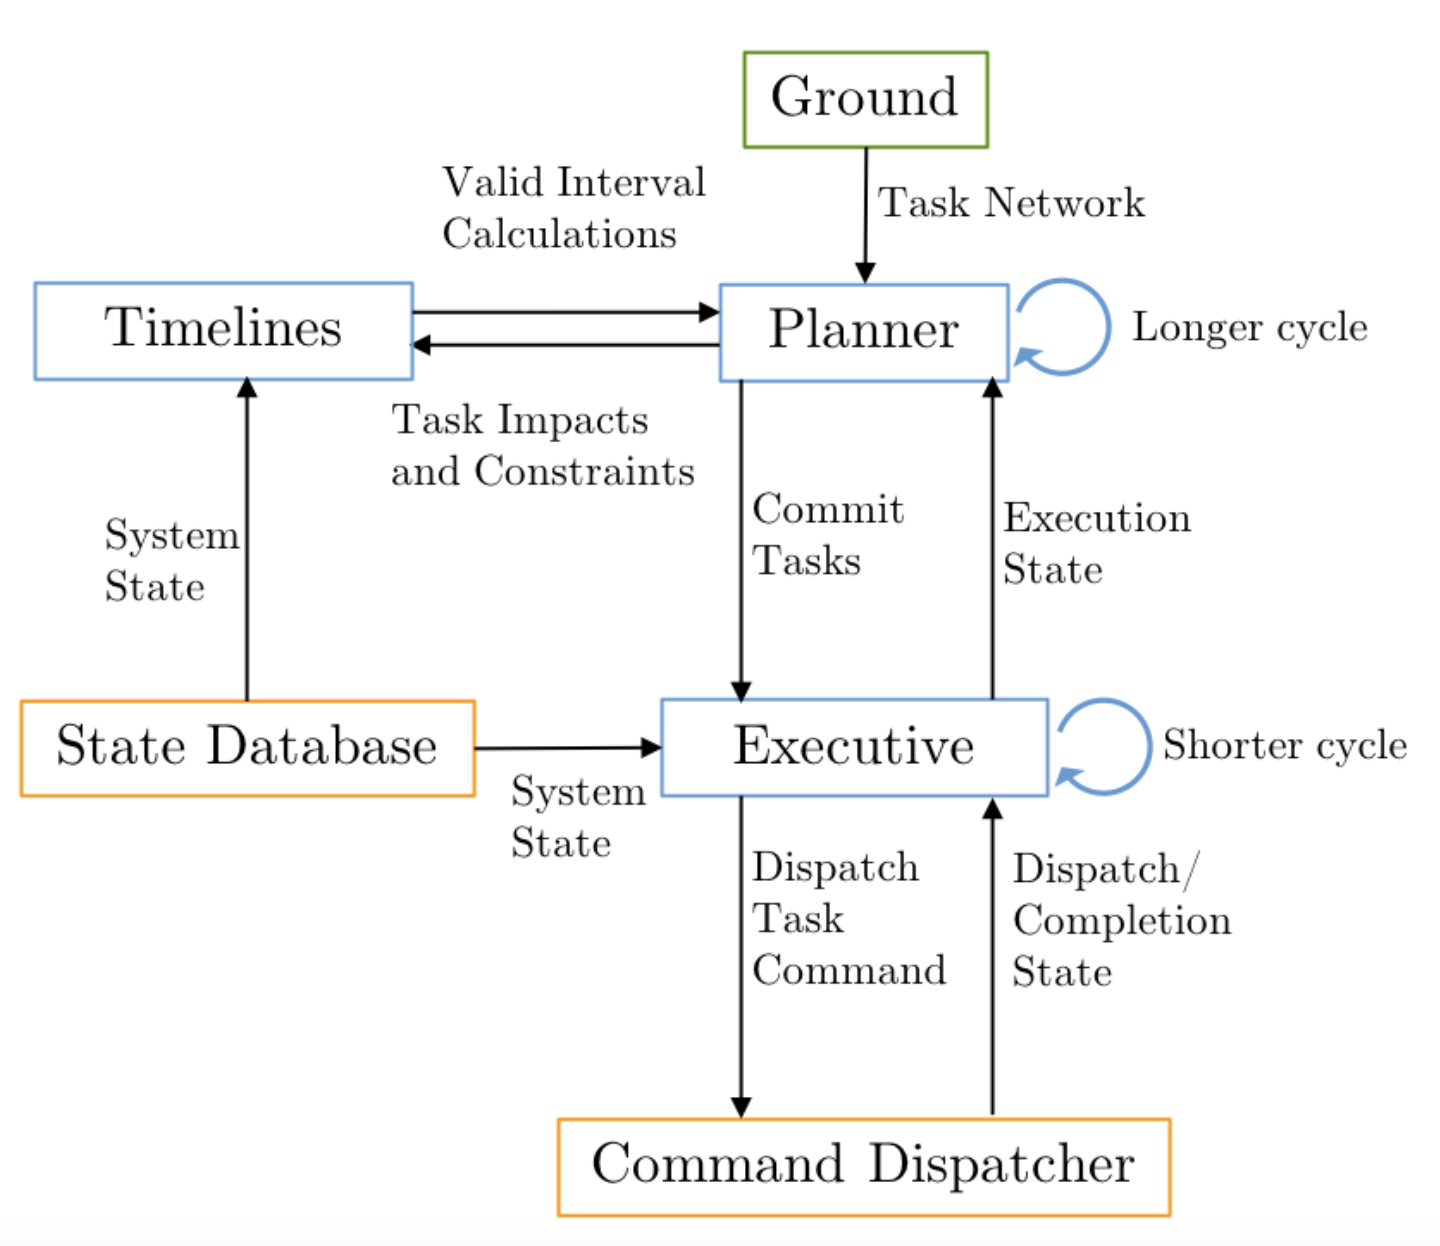
\includegraphics[width=\textwidth]{figures/mexec.png}
\end{column}
\begin{column}{0.46\textwidth}
JPL's onboard planner and executive. Ground uplinks a {\bf task network}: tasks,
the {\bf timelines} they read and write, and the constraints between them.

\vspace{0.3cm}
\mexec{} schedules it onboard and repairs the plan as it executes.

\pause
\vspace{0.3cm}
{\bf The question:} before we uplink a task network, can we know that it can be
scheduled at all, and that every schedule it admits is safe?
\end{column}
\end{columns}

\end{frame}

%----------------------------------------
\begin{frame}
  \frametitle{\tasksat{}} \small

A DSL for task networks, as close as we could get to \mexec{}'s concepts and
semantics, plus temporal logic. Solved with \zthree{}.

\vspace{0.3cm}
{\centering\scriptsize
\setlength{\tabcolsep}{4pt}
\renewcommand{\arraystretch}{1.3}
\begin{tabular}{llc}
\toprule
{\bf Question} & & {\bf Form} \\
\midrule
Validity      & Is there any schedule? (the planning problem) & $\exists i\, \exists s\, .\ \mathit{valid}(i,s)$ \\
Properties    & Is every schedule safe?                         & $\forall i\, \forall s\, .\ \mathit{valid}(i,s) \Rightarrow \varphi$ \\
\pause
Realizability & Is there a schedule from {\em every} initial state? & $\forall i\, \exists s\, .\ \mathit{valid}(i,s)$ \\
Compositional & Does it hold for {\em any} number of repetitions?  & $\{P\}\,S\,\{P\} \Rightarrow \forall N.\{P\}\,S^N\{P\}$ \\
\bottomrule
\end{tabular}\par}

\vspace{0.3cm}
$i$ is an initial state, $s$ a schedule.

\end{frame}

%----------------------------------------
\begin{frame}
  \frametitle{The pipeline} \small

{\centering
\begin{tikzpicture}[
  font=\scriptsize, >=Stealth, node distance=0.45cm,
  b/.style={draw, rounded corners=2pt, align=center, minimum height=0.8cm,
            minimum width=1.7cm, fill=blue!5},
  zz/.style={b, fill=green!10, draw=green!45!black},
  o/.style={b, fill=yellow!10}
]
  \node[o] (tn) {\tt .tn\\{\tiny spec}};
  \node[b, right=of tn]  (p) {parse};
  \node[b, right=of p]   (t) {transform\\{\tiny sugar, instances}};
  \node[b, right=of t]   (w) {well-formed\\+ lint};
  \node[b, below=0.9cm of w] (e) {SMT encode\\{\tiny zones}};
  \node[zz, left=of e]    (s) {\zthree{}};
  \node[o, left=of s]    (r) {schedule\\{\tiny or UNSAT core}};
  \node[o, left=of r]    (v) {Gantt, web UI,\\JSON};
  \draw[->] (tn) -- (p); \draw[->] (p) -- (t); \draw[->] (t) -- (w);
  \draw[->] (w) -- (e);  \draw[->] (e) -- (s); \draw[->] (s) -- (r); \draw[->] (r) -- (v);
\end{tikzpicture}\par}

\vspace{0.5cm}
\begin{itemize}
\item Much of the language is {\bf sugar}: task ranges, sessions, mutex, auto-instantiation
      are all flattened before encoding.
\item The encoding is {\bf quantifier-free}: one formula, one solver call per question.
\item Python, PLY, \zthree{}, Flask. Open source: {\tt github.com/nasa-jpl/tasksat}
\end{itemize}

\end{frame}
